\section{Benutzeroberfläche}
%[TODO: remove this link] https://tex.stackexchange.com/questions/442077/is-it-possible-to-use-svg-images-with-overleaf

Es handelt sich hier lediglich um Entwürfe. Dementsprechend sind Änderungen vorbehalten, insbesondere im Design. Auch kann das finale Produkt leicht von diesen Entwürfen abweichen, auch wenn keine größere Änderung vorgenommen wird.\\
Man beachte, das in den Entwürfen auch Funktionalität zu sehen ist, welche aus Wunschkriterien stammen. Die auf diesen Entwürfen enthaltenen Markierungen (Kreise mit Zahlen und rotem Rand) dienen lediglich zur Lokalisierung der Erläuterungen und werden nicht im finalen Produkt enthalten sein.
\subsection{Anmeldung}
\label{pages:login}
\begin{figure}[H]
    \centering
    \includegraphics[width=\textwidth]{images-interface/v4_interface/login_page_4.pdf}
    \caption{Anmeldung}
    \label{fig:login}
\end{figure}
Auf dieser Seite kann sich ein Nutzer mit einem bereits vorhandenen Konto anmelden. Diese Seite wird einem nicht angemeldetem Nutzer standardmäßig bei Aufruf des Web-Interfaces angezeigt. Ist ein Nutzer bereits angemeldet, so wird er zur \hyperref[pages:job-table]{Job-Tabelle} weitergeleitet.\\
\newpage
\textbf{Erläuterungen}
\begin{itemize}
    \item[1)] Die Schaltfläche \enquote{Register} leitet zur \hyperref[pages:register]{Registrierungsseite} weiter.
    \item[2)] Die Schaltfläche \enquote{Log in} meldet den Nutzer bei korrekt eingegebenen Daten an und leitet ihn zur \hyperref[pages:job-table]{Job-Tabelle} weiter.
\end{itemize}

\subsection{Registrierung}
\label{pages:register}
\begin{figure}[H]
    \centering
    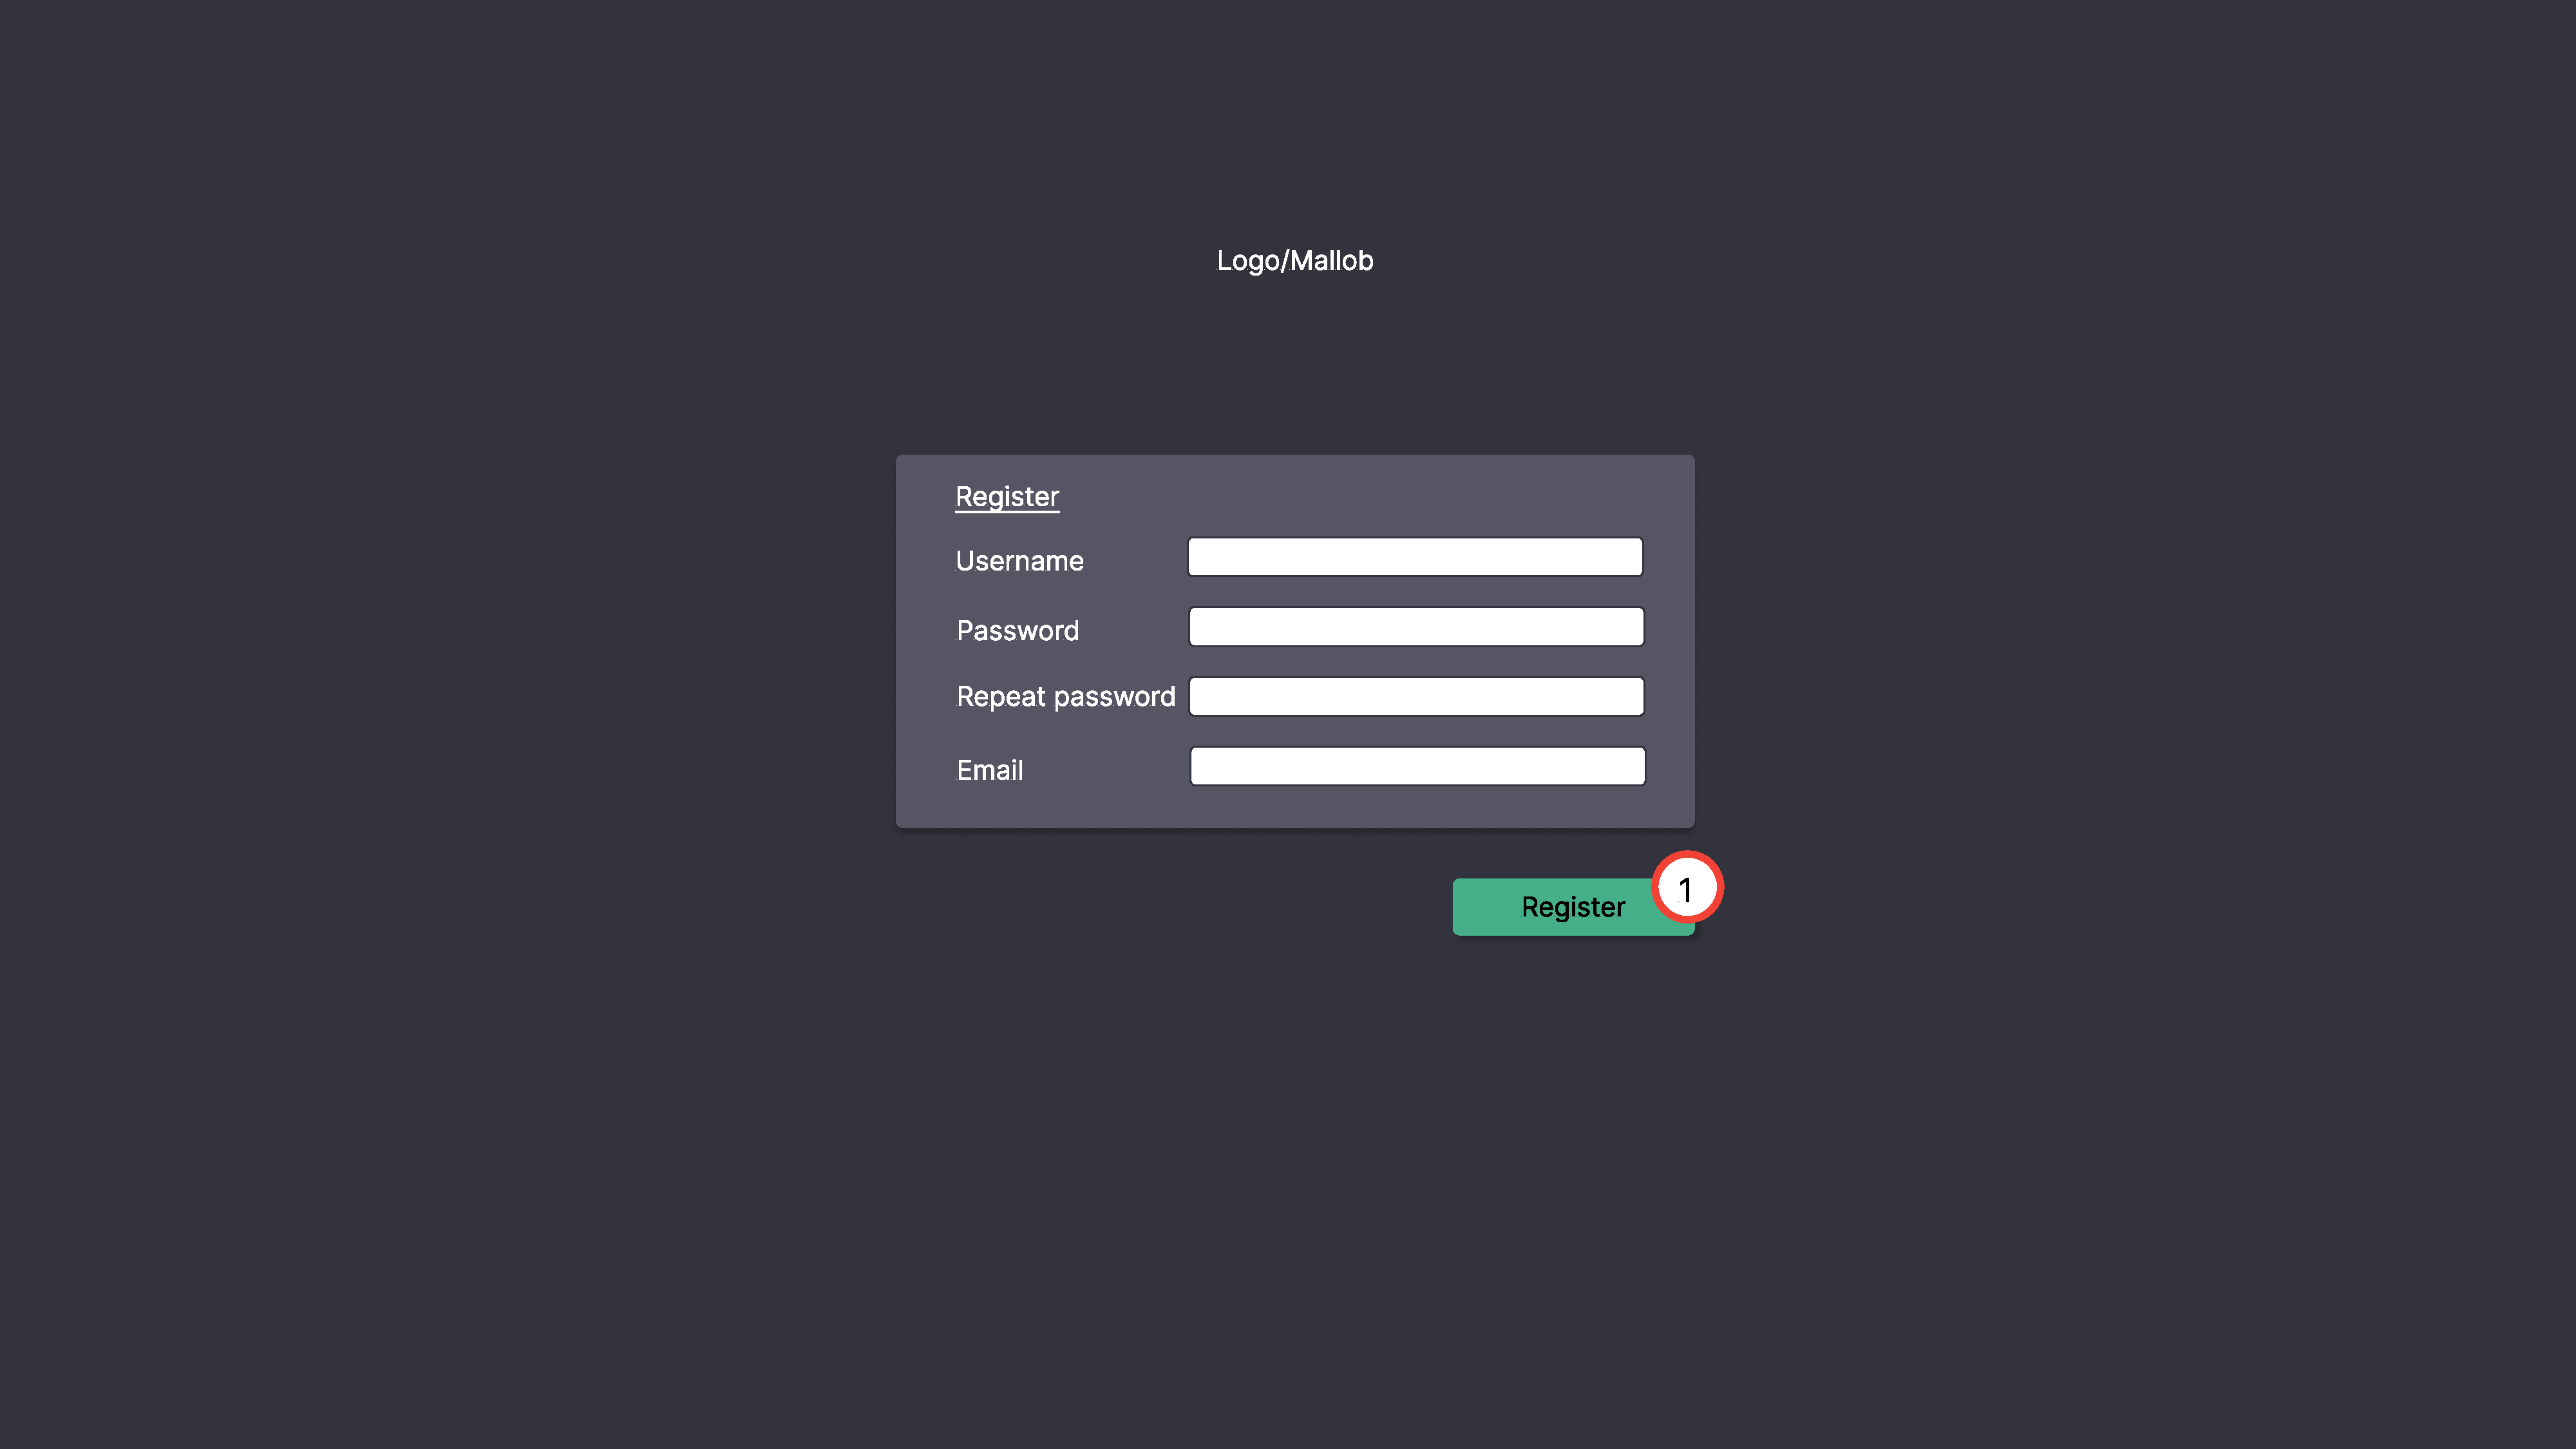
\includegraphics[width=\textwidth]{images-interface/v4_interface/register_page_4.pdf}
    \caption{Registrierung}
    \label{fig:register}
\end{figure}
Auf dieser Seite kann sich eine Person registrieren. Sind die Eingabedaten korrekt, wird ein neues vorläufiges Konto mit den entsprechenden Daten erstellt. \\


\textbf{Erläuterungen}
\begin{itemize}
    \item[1)] Die Schaltfläche \enquote{Register} registriert den Nutzer und leitet in zur \hyperref[pages:visualization]{Visualisierung} weiter, da sein Konto direkt nach der Registrierung noch nicht verifiziert ist und er somit ohnehin noch keine Jobs einreichen kann.
\end{itemize}



\newpage
\subsection{Job-Tabelle}
\label{pages:job-table}
\begin{figure}[H]
    \centering
    \label{fig:job-table-col}
    \includegraphics[width=\textwidth]{images-interface/v4_interface/job_table_page_collapsed_4.pdf}
    \caption{Job—Tabelle}
    
    \label{fig:job-table-exp}
    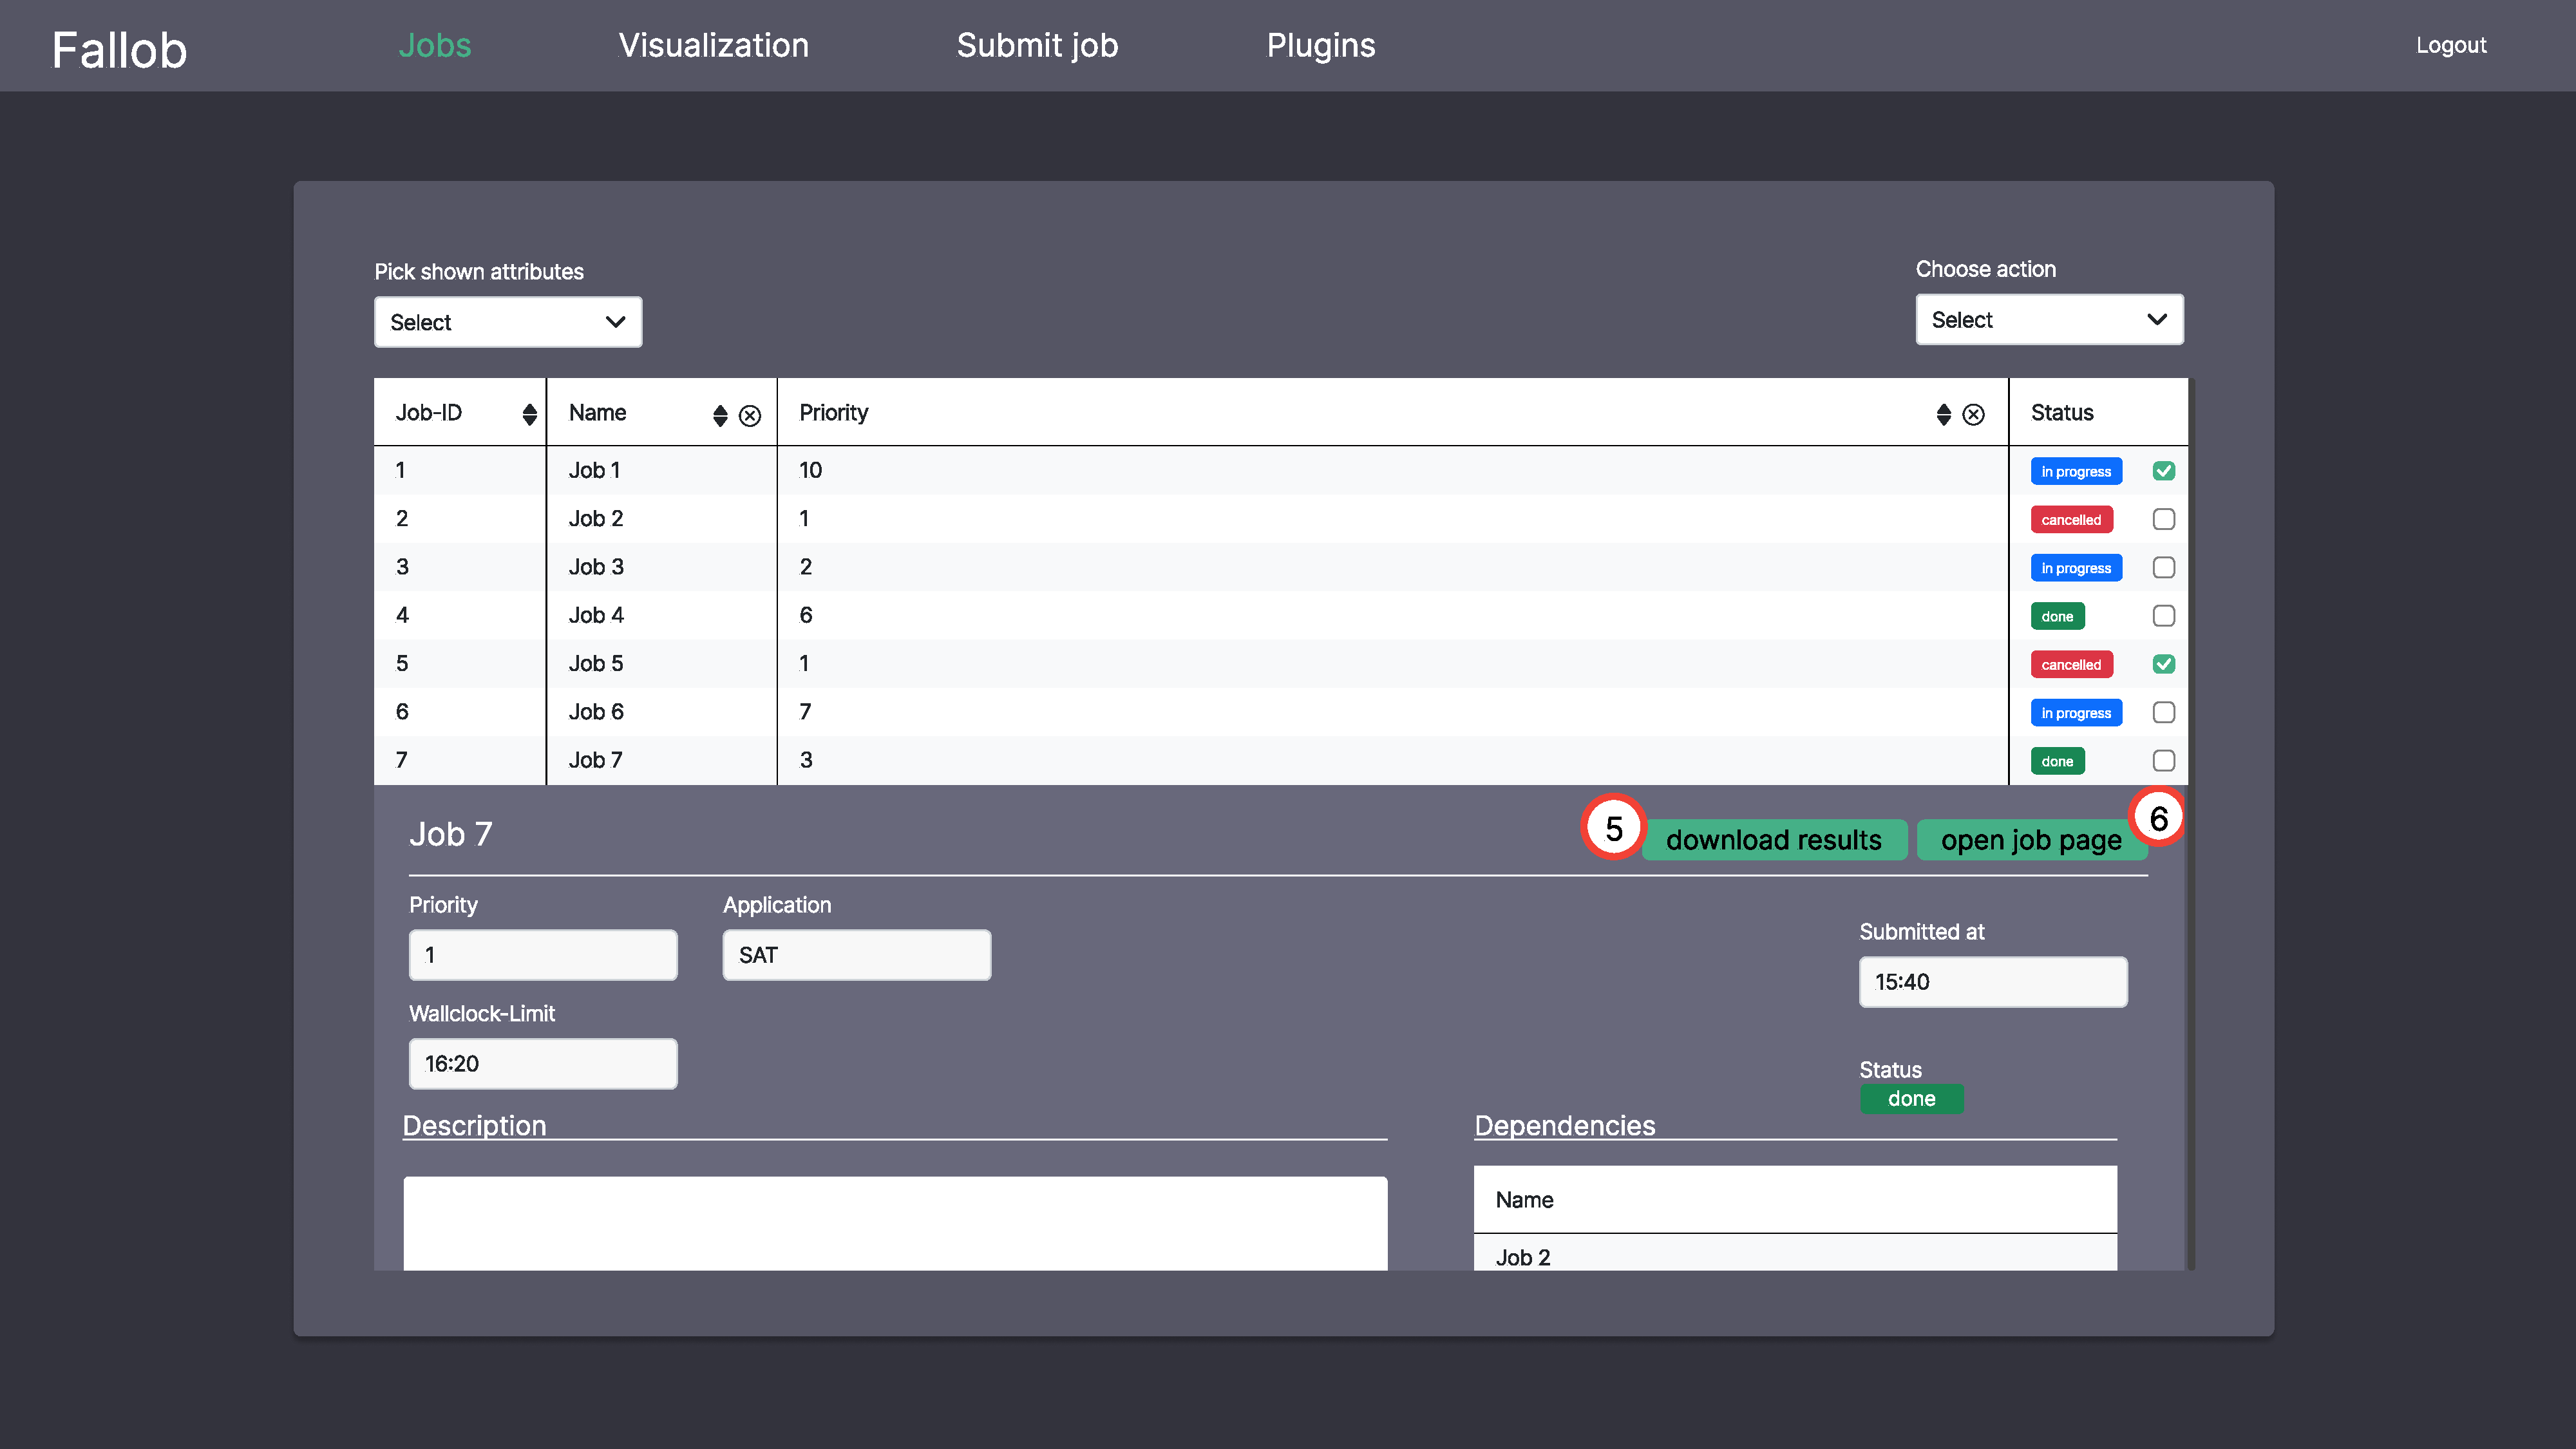
\includegraphics[width=\textwidth]{images-interface/v4_interface/job_table_expanded_4.pdf}
    \caption{Job-Tabelle mit aufgeklappter Ansicht für einen Job}
    
\end{figure}
Auf dieser Seite gibt es eine Übersicht über die Jobs, die der Nutzer bereits eingereicht. Das ganze findet in tabellarischer Form statt. Die Spalten Job-ID und Status sowie die Spalte mit den Checkboxen werden immer dargestellt, die restlichen Spalten sind alle optional auswählbar.\\
Die in \hyperref[fig:job-table-exp]{Abbildung 12} zu sehende aufgeklappte Ansicht wird angezeigt, wenn der Nutzer auf eine Zeile eines Jobs klickt. Zu jedem Zeitpunkt ist immer nur maximal ein Job aufgeklappt. Sollte bereits ein Job aufgeklappt sein, so wird er wieder eingeklappt, wenn ein anderer aufgeklappt wird.\\

\textbf{Erläuterungen}
\begin{itemize}
    \item[1)] Über dieses Dropdown-Menü können gemäß \hyperref[FA:Web-Interface:Hinzufügen von Spalten]{FA2120} weitere Attribute in der Tabelle angezeigt werden. Im Dropdown-Menü werden nur Attribute angezeigt, die noch nicht in der Tabelle angezeigt werden.
    \item[2)] Über dieses Dropdown-Menü kann eine Aktion (siehe \hyperref[FA:Web-Interface:Abbruch mehrerer Jobs auf einmal]{FA2050} und \hyperref[FA:Web-Interface:herunterladen mehrerer Ergebnisse auf einmal]{FA2070}) durchgeführt werden, welche auf alle mit der Checkbox ausgewählten Jobs angewandt wird.
    \item[3)] Über diese Checkboxen kann ein Job für eine Aktion nach Punkt Zwei dieser Liste ausgewählt werden.
    \item[4)] Über das Symbol mit den beide Dreiecken kann die entsprechende Spalte gemäß \hyperref[FA:Web-Interface:Sortieren der Tabelle]{FA2130} sortiert werden. Mit dem Kreuz-Symbol kann die Spalte gemäß \hyperref[FA:Web-Interface:Entfernen von Spalten]{F2150} wieder aus der Tabelle gelöscht werden.
    \item[5)] Über diese Schaltfläche kann das Ergebnis gemäß \hyperref[FA:Web-Interface:Herunterladen eines einzelnen Ergebnisses]{FA2060} heruntergeladen werden. Man beachte, dass diese Schaltfläche nur bei abgeschlossenen Jobs verfügbar ist. Bei laufenden Jobs bietet sie die Möglichkeit, den Job abzubrechen. Bei abgebrochenen Jobs bietet sie die Möglichkeit, den Job neuzustarten.
    \item[6)] Über diese Schaltfläche wird der Nutzer zur entsprechenden \hyperref[pages:job-page]{Job-Seite} des Jobs weitergeleitet.
\end{itemize}

\newpage
\subsection{Job einreichen}
\label{pages:submit-job}
\begin{figure}[H]
    \centering
    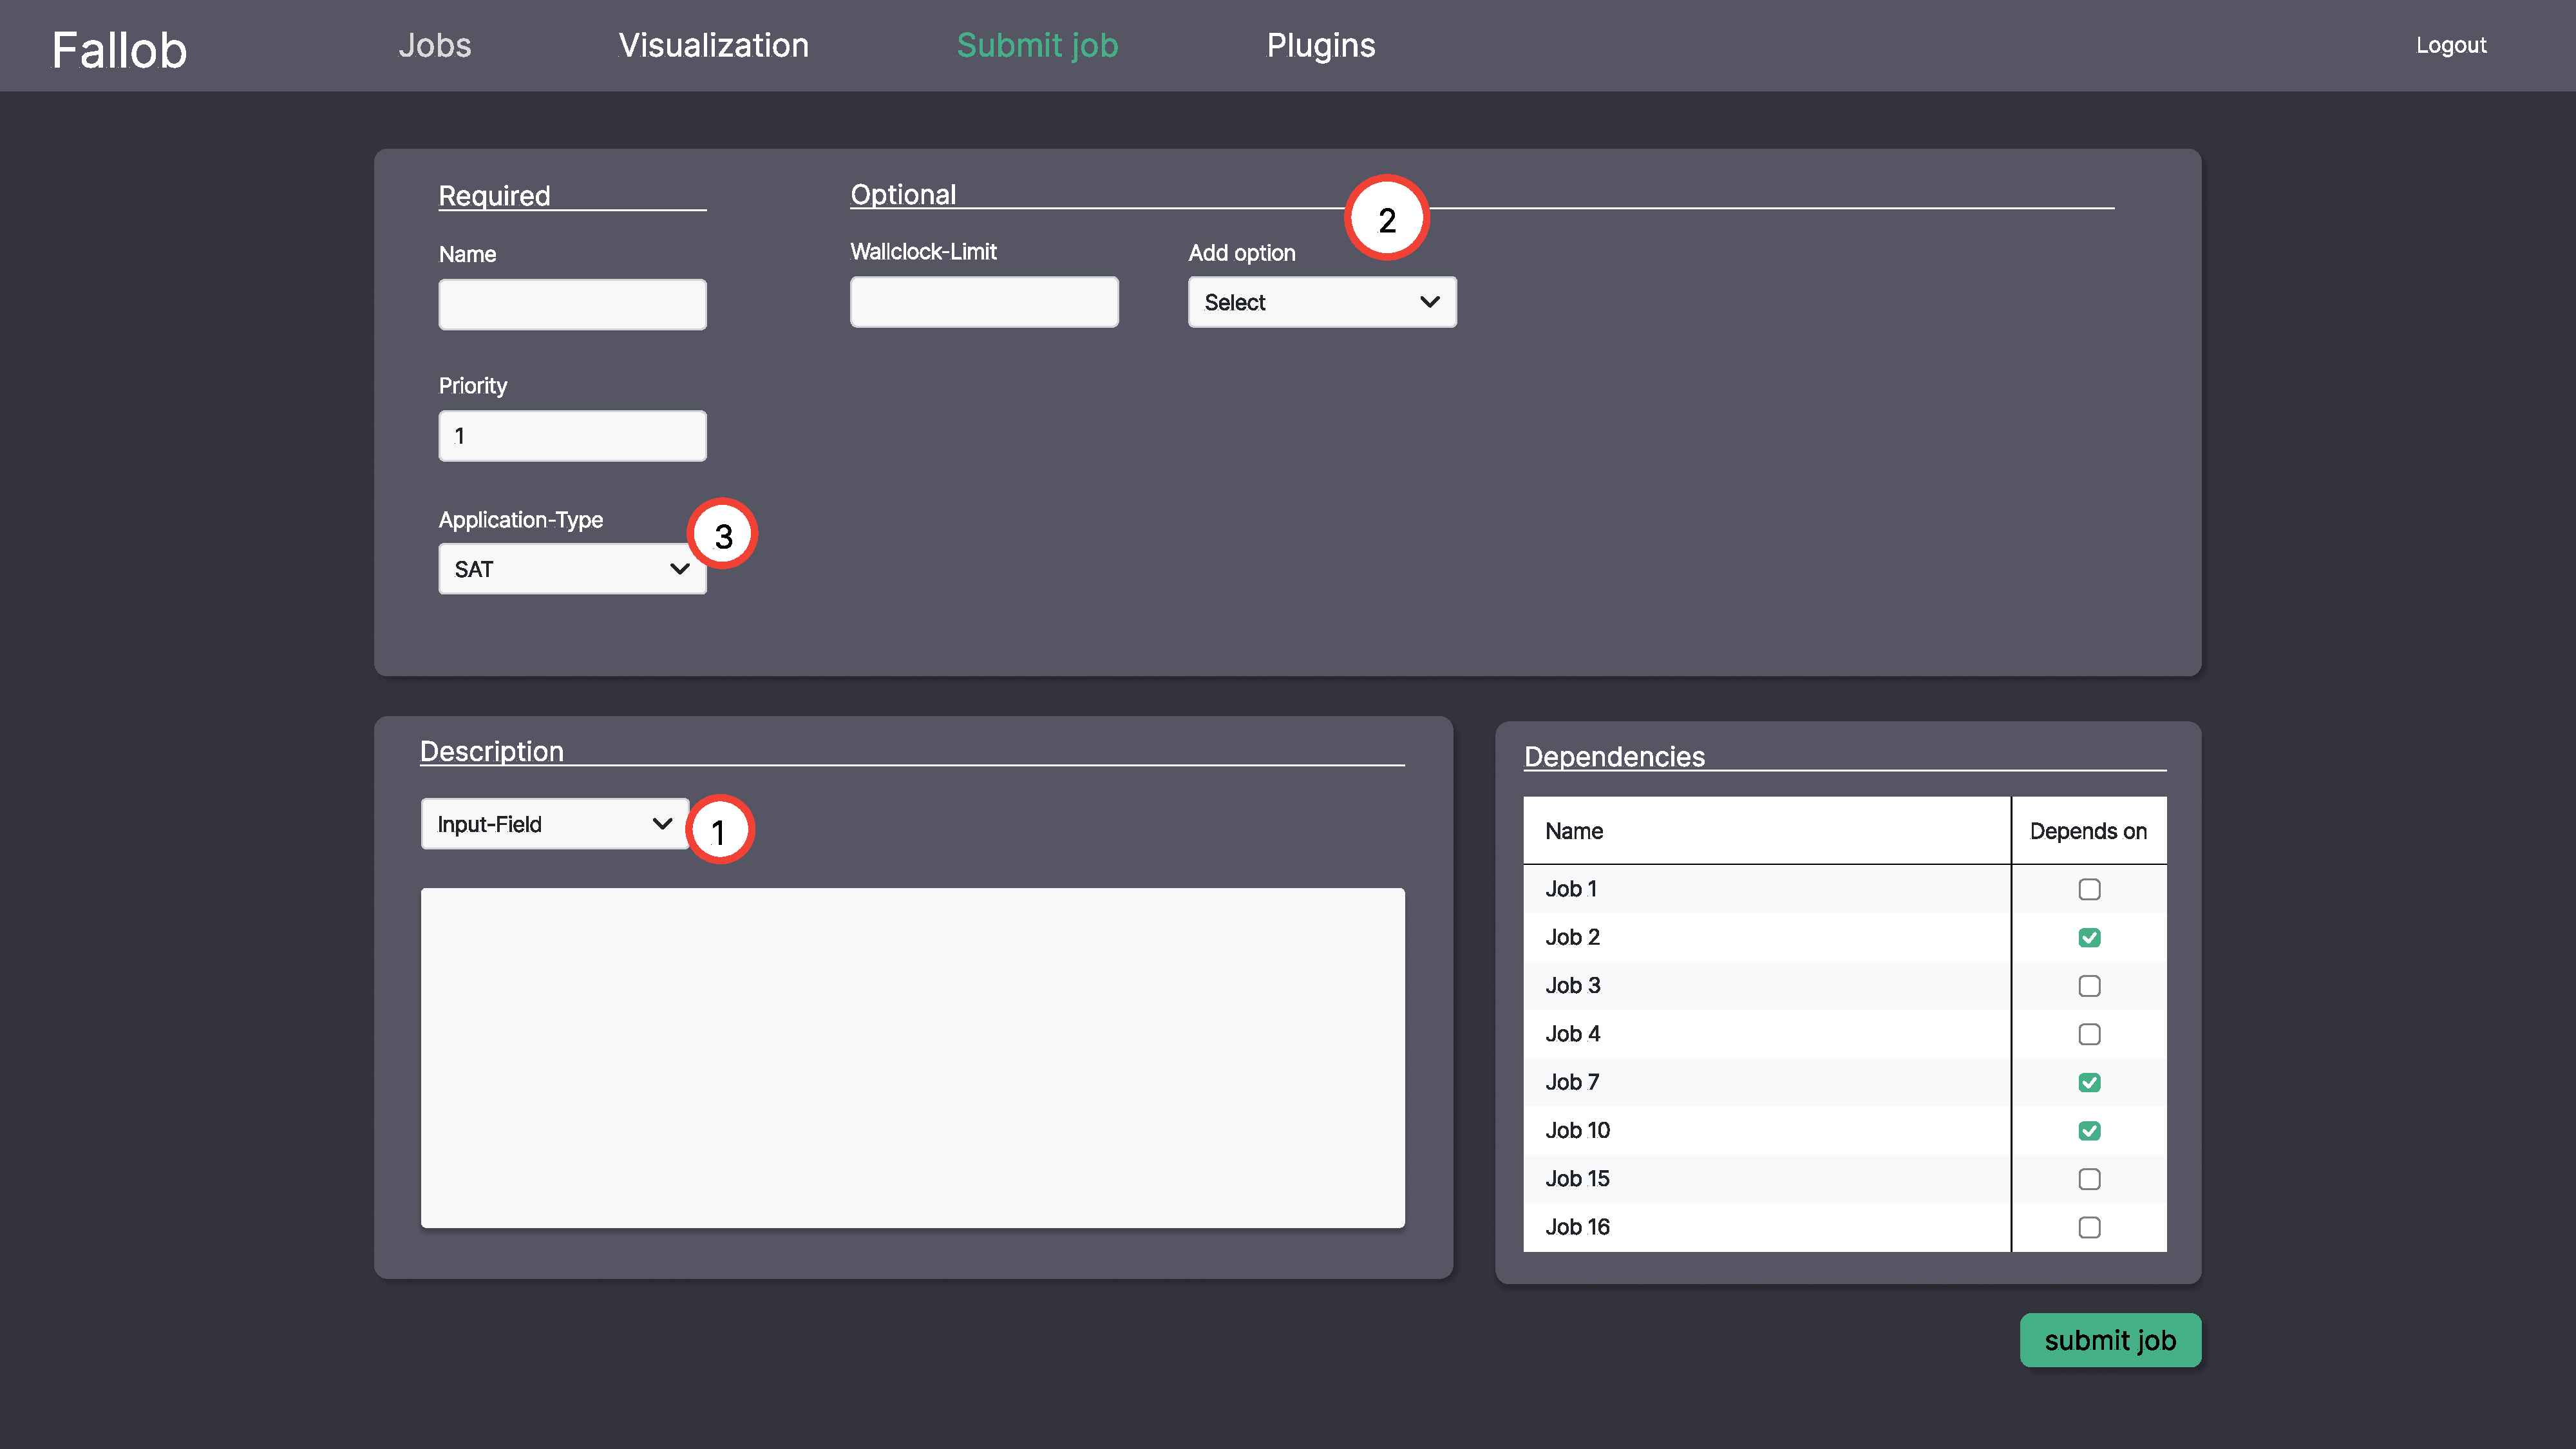
\includegraphics[width=\textwidth]{images-interface/v4_interface/submit_job_page_4.pdf}
    \caption{Einreichen neuer Jobs}
    \label{fig:submit-job}
\end{figure}
Auf dieser Seite können neue Jobs eingereicht werden. Es gibt die Möglichkeit, die Job-Parameter korrekt einzustellen, die Job-Beschreibung hinzuzufügen sowie die Möglichkeit, Abhängigkeiten zu anderen Jobs anzugeben. \\

\textbf{Erläuterungen}
\begin{itemize}
    \item[1)] Mit diesem Dropdown-Menü kann gemäß \hyperref[FA:Web-Interface:Job einreichen]{FA2030} gewählt werden, auf welchem Wege die Job-Beschreibung übermittelt wird. Die Job-Beschreibung muss auf genau einem dieser Wege übermittelt werden.
    \item[2)] Mit diesem Dropdown-Menü können weitere, optionale Job-Parameter gemäß \hyperref[FA:Web-Interface:Job einreichen]{FA2030} ausgewählt werden. 
    \item[3)] Mit diesem Dropdown-Menü kann der Job-Typ ausgewählt werden. Zur Auswahl stehen SAT, DUMMY und KMEANS.
\end{itemize}

\newpage
\subsection{Job-Seite}
\label{pages:job-page}
\begin{figure}[H]
    \centering
    \includegraphics[width=\textwidth]{images-interface/v4_interface/job_info_page_4.pdf}
    \caption{Info-Seite eines Jobs}
    \label{fig:job-page}
\end{figure}
Diese Seite bietet eine Übersicht über einen einzelnen Job. Es werden die Job-Konfiguration, die Job-Beschreibung, die Abhängigkeiten, den Zeitpunkt des Einreichens und der aktuelle Zustand angezeigt. Weiterhin besteht die hier die Möglichkeit, das Ergebnis eines abgeschlossenen Jobs herunterzuladen. Man gelangt zu dieser Seite gemäß \hyperref[FA:Web-Interface:Einsehen von Job-Informationen]{F2140}.

\textbf{Erläuterungen}
\begin{itemize}
    \item[1)] Hier werden möglicherweise auch noch weitere, für diesen Job gewählten optionale Parameter angezeigt.
\end{itemize}

\newpage
\subsection{Visualisierung}
\label{pages:visualization}
\begin{figure}[H]
    \centering
    \includegraphics[width=\textwidth]{images-interface/v4_interface/visualization_page_4.pdf}
    \caption{Visualisierung des Systems}
    \label{fig:visualization-page}
\end{figure}
Diese Seite visualisiert den Systemzustand. Im linken Panel ist hierbei die Ansicht der Prozesse und zugeordneten Jobs zu sehen. Das Panel rechts ist zunächst leer. Es wird, wie hier zu sehen, erst mit Informationen gefüllt, wenn der Nutzer auf einen Prozess im Panel links auswählt. Dann werden zu diesem einen Prozess der Rank, die größe des Binär-Baumes, die größe des Ausgewählten Subbaumes und Informationen über den Nutzer. (siehe Punkt 4 der Erläuterungen) //

\textbf{Erläuterungen}
\begin{itemize}
    \item[1)] Verwendet Mallob zu viele Prozesse, so erscheint eine Scrollbar, mithilfe derer die Ansicht vertikal verschoben werden kann.
    \item[2)] Hier findet die eigentliche Visualisierung gemäß \hyperref[FA:Web-Interface:Verifizieren eines Kontos]{FA3000} statt. In diesem Falle ist ein Administrator angemeldet (erkennbar daran, das Schaltfläche "Administration" in der Navigations-Leiste sichbtbar ist), daher sind alle Jobs farbig und nicht in Grautönen. Für einen nicht-Administrator werden Jobs von anderen Nutzern pseudonymisiert und grau angezeigt.
    \item[3)] Hier wird gemäß \hyperref[FA:Visualisierung:Anzeigen des Binaerbaumes für einen Job]{FA3010} der Binärbaum eines Jobs angezeigt.
    \item[4)] Informationen über den Nutzer, dem der Job gehört. Wird nur angezeigt, da ein Administrator angemeldet ist.
\end{itemize}

%Anmerkung zur Plugin einsicht; Evtl oben in der Querleiste ein Reiter "Plugins" und das dann als Dropdown menü für alle hinzugefügtten Plugins machen. Das macht die Seite stabiler für viele Plguins
% gute idee, schaff ich heute aber nicht mehr

\subsection{Plugin-Ansicht}
\label{pages:plugin}
\begin{figure}[H]
    \centering
    \includegraphics[width=\textwidth]{images-interface/v4_interface/plugin_page_4.pdf}
    \caption{Generische Ansicht für Plugins}
    \label{fig:plugin-page}
\end{figure}
Diese Seite stellt die generische Ansicht für Plugins dar. Um zu dieser Seite zu gelangen, kann man oben über das Dropdown-Menü in der Navigations-Leiste ein verfügbares Plugin auswählen. Gibt es keine Plugins, so wird das Dropdown-Menü nicht angezeigt. \\

\textbf{Erläuterungen}
\begin{itemize}
    \item[1)] Hier kann der Job ausgewählt werden, welcher vom Plugin verarbeitet wird.
    \item[2)] Diese Fläche steht dem Plugin frei zur Darstellung zur Verfügung.
\end{itemize}

\newpage
\subsection{Administration}
\label{pages:admin}
\begin{figure}[H]
    \centering
    \includegraphics[width=\textwidth]{images-interface/v4_interface/admin_page_4.pdf}
    \caption{Seite für Administratoren zur Verwaltung des Systems}
    \label{fig:admin-page}
\end{figure}
Diese Seite dient der Verwaltung des Systems. Sie ist nur für angemeldete Administratoren sichtbar. \\

\textbf{Erläuterungen}
\begin{itemize}
    \item[1)] Hier wird kann die Instanz von Mallob verwaltet.
    \item[2)] Hier werden gemäß \hyperref[FA:Web-Interface:Anzeigen von Warungen und Fehlermeldungen]{FA2110} Warnungen und Fehlermeldungen angezeigt, die Mallob ausgibt.
    \item[3)] Hier werden gemäß \hyperref[]{[TODO]} Diagnose-Daten angezeigt.
\end{itemize}

%\newpage
%\subsection{Funktionen}
%\begin{itemize}
%    \item /B010/ Es sind zwei Sichten zu unterscheiden: die des Admins, die des Benutzers. 
%    \item /B020/ Benutzer können Funktionen F10, F20, F30 jederzeit nach dem Einloggen aufrufen.
%    \item /B030/ Jeder Benutzer fängt auf der Login/Register-Seite an.
%    \item /B040/ Sobald der Benutzer eingeloggt wird, sieht er die Startseite.
%    \item /B050/ Jeder Nutzer kann seine Jobs anhand der Aufwand auf das Kern unterscheiden (z.B Farbe, Größe usw.)
%    \item /B060/ Admins können alle Funktionen, die die Benutzer können.
%    \item /B070/ Unterschiedliche Benutzer und ihre Befugnisse sollen entsprechend behandelt werden (nicht-funktionale Anforderung?).
%    \item /B080/ Die Bedienungsoberfläche ist auf Mausbedienung auszulegen; eine Bedienung ohne Maus muss aber auch möglich sein. ([TODO] Bediengung ohne Maus auf jeden Fall wunschkriterium oder vlt sogar gar nicth, auf jeden Fall mal fragen, hört sich kompliziert und nicht wirklich notwendig an)
%\end{itemize}